W ramach niniejszego dodatku zostanie przedstawiona szczegółowa dokumentacja
protokołu komunikacyjnego zaprojektowanego na potrzeby sterowania robotem Dark
Explorer przy użyciu technologii bluetooth. Zasady przesyłania
poleceń wraz z ogólnym zarysem sposobu podziału komunikatów został szczegółowo
omówiony w ramach rozdziału \ref{sec:ch05_s01_comm}. W tej części zaprezentowane
zostaną wszystkie dostępne polecenia sterujące wraz z~przykładami
formatów odpowiedzi w przypadku prawidłowego wykonania polecenia.

\section{Komunikaty sterujące}
\subsection{Sterowanie silnikami}
\begin{figure}[h!]
 \centering
 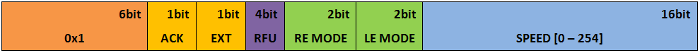
\includegraphics[width=\textwidth]{../images/appendix/cmd_0x01.png}
 \caption{Schemat ramki odpowiedzialnej za sterowanie silnikami} 
 \label{fig:CMD_0x01}
\end{figure}

\begin{basedescript}{\desclabelstyle{\pushlabel}\desclabelwidth{25mm}}
\setlength{\parsep}{0pt}
\setlength{\itemsep}{0mm}
\setlength{\parskip}{0pt}
\item[ACK]
	Wartość 0x1 jeśli komunikat wymaga potwierdzenia
\item[EXT] 
	Wartość 0x1 jeśli komunikat zawiera dane o mocy silników
\item[RFU] 
	Bity zarezerwowane do przyszłego użycia
\item[RE MODE] 
	Tryb pracy silników prawych (0x0 - stop, 0x1 - wprost, 0x2 - wstecz)
\item[LE MODE] 
	Tryb pracy silników lewych (0x0 - stop, 0x1 - wprost, 0x2 - wstecz)
\item[SPEED] 
	Moc silników. Wartość z zakresu [0 - 254]
\end{basedescript}

\subsection{Sterowanie serwomechanizmem}
\begin{figure}[h!] 
 \centering
 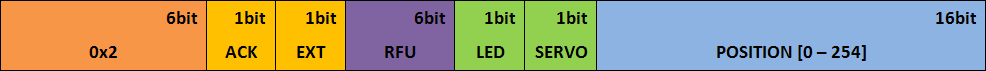
\includegraphics[width=\textwidth]{../images/appendix/cmd_0x02.png}
 \caption{Schemat komunikatu odpowiedzialnego za sterowanie serwomechanizmem}
 \label{fig:CMD_0x02}
\end{figure}

\begin{basedescript}{\desclabelstyle{\pushlabel}\desclabelwidth{25mm}}
\setlength{\parsep}{0pt}
\setlength{\itemsep}{0mm}
\setlength{\parskip}{0pt}
\item[ACK]
	Wartość 0x1 jeśli komunikat wymaga potwierdzenia
\item[EXT] 
	Wartość 0x1 jeśli komunikat zawiera dane o położeniu
\item[RFU] 
	Bity zarezerwowane do przyszłego użycia
\item[LED] 
	Wartość 0x1 jeśli status diody LED ma zostać zmieniony na przeciwny
\item[SERVO] 
	Wartość 0x1 jeśli stan serwomechanizm ma zostać zmieniony na przeciwny
\item[POSITION] 
	Pozycja (kąt) pod jakim ma zostać ustawiona wieżyczka z kamerą.
\end{basedescript}

\subsection{Akwizycja obrazu z kamery}
\begin{figure}[h!] 
 \centering
 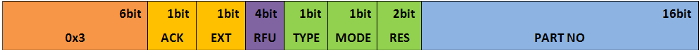
\includegraphics[width=\textwidth]{../images/appendix/cmd_0x03.png}
 \caption{Schemat komunikatu odpowiedzialnego za akwizycję obrazu z kamery}
 \label{fig:CMD_0x03}
\end{figure}

\begin{basedescript}{\desclabelstyle{\pushlabel}\desclabelwidth{25mm}}
\setlength{\parsep}{0pt}
\setlength{\itemsep}{0mm}
\setlength{\parskip}{0pt}
\item[ACK]
	Wartość 0x1 jeśli komunikat wymaga potwierdzenia
\item[EXT] 
	Wartość 0x1 jeśli komunikat zawiera dane o położeniu
\item[RFU] 
	Bity zarezerwowane do przyszłego użycia
\item[TYPE] 
	Typ operacji (0x0 - akwizycja obrazu, 0x1 transmisja pobranego obrazu)
\item[MODE] 
	Tryb pracy kamery (0x0 - odcienie szarości, 0x1 - kolor)
\item[RES] 
	Identyfikator rozmiaru obrazu według następującej specyfikacji:
	\begin{desc}
	\item[0x0] - 160x120
	\item[0x1] - 320x240
	\item[0x2] - 640x480
	\end{desc} 
\end{basedescript}

\subsection{Sterowanie czujnikami}
\begin{figure}[h!] 
 \centering
 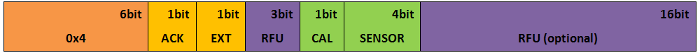
\includegraphics[width=\textwidth]{../images/appendix/cmd_0x04.png}
 \caption{Schemat komunikatu odpowiedzialnego za odpytywanie czujników}
 \label{fig:CMD_0x04}
\end{figure}

\begin{basedescript}{\desclabelstyle{\pushlabel}\desclabelwidth{25mm}}
\setlength{\parsep}{0pt}
\setlength{\itemsep}{0mm}
\setlength{\parskip}{0pt}
\item[ACK]
	Wartość 0x1 jeśli komunikat wymaga potwierdzenia
\item[EXT] 
	Wartość 0x1 jeśli komunikat zawiera dane rozszerzone
\item[RFU] 
	Bity zarezerwowane do przyszłego użycia
\item[CAL] 
	Ustawienie wartości 0x1 spowoduje uruchomienie procedury kalibrującej
	dla sensora podanego w sekcji SENSOR
\item[SENSOR] 
	Unikalny identyfikator typu pomiaru (czujnika) który ma zostać przeprowadzony,
	według następującej specyfikacji:
	\begin{desc}
	\item[0x0] - pomiar napięcia na baterii
	\item[0x1] - pomiar temperatury
	\item[0x2] - pomiar przyspieszenia statycznego
	\item[0x3] - informacje o odległości od najbliższej przeszkody
	\item[0x4] - informacje o położeniu na podstawie magnetometru
	\end{desc}
\end{basedescript}


\section{Komunikaty specjalne}